\documentclass{article}
\usepackage{graphicx}
\usepackage{subfigure}
\usepackage{multirow}
\usepackage{wrapfig}
\usepackage{amssymb}
\usepackage{amsfonts, amsmath}
\usepackage{amsmath}
\usepackage{mathrsfs}
\usepackage{enumerate}
\usepackage[bookmarks=true]{hyperref}
\usepackage[acronym]{glossaries}
\usepackage{bookmark}
\usepackage{amssymb,amsmath,amsthm,amsfonts}
\usepackage{mathrsfs}
\usepackage{dsfont}
\usepackage{enumerate}

%\newtheorem{mdef}{Definition}
%\newtheorem{theorem}{Theorem}
\newcommand{\eqsplit}[2]{
  \begin{equation}\label{#2}
    \begin{split}
      #1
    \end{split}
  \end{equation}}
\newcommand{\eqnsplit}[1]{
  \begin{eqnarray*}
    #1
  \end{eqnarray*}}
\newcommand{\tran}[1]{
  \tilde{#1}
}
\newcommand{\td}[2]{
  \frac{d #1}{d #2}
}
\newcommand{\pd}[2]{
  \frac{\partial #1}{\partial #2}
}
\newcommand{\ppd}[2]{
  \frac{\partial^2 #1}{\partial #2^2}
}
\newcommand{\pdd}[3]{
  \frac{\partial^2 #1}{\partial #2 \partial #3}
}
\newcommand{\otd}[1]{
  \frac{d}{d #1}
}
\newcommand{\opd}[1]{
  \frac{\partial}{\partial #1}
}
\newcommand{\oppd}[1]{
  \frac{\partial^2}{\partial #1^2}
}
\newcommand{\opdd}[2]{
  \frac{\partial^2}{\partial #1 \partial #2}
}
\newcommand{\ket}[1]{
  |#1\rangle
}
\newcommand{\bra}[1]{
  \langle#1|
}
\newcommand{\inn}[1]{
  \langle#1\rangle
}
\newcommand{\mean}[1]{
  \langle#1\rangle
}
\newcommand{\tr}{
  \text{tr}\,
}
\newcommand{\re}{
  \text{Re}\,
}
\newcommand\im{
  \text{Im}\,
}
\newcommand{\var}{
  \text{var}
}
\newcommand{\arcsinh}{
  \sinh^{-1}
}
\newcommand{\arccosh}{
  \cosh^{-1}
}
\newcommand{\erfc}{
  \text{erfc}
}
\newcommand{\E}{
  \mathbb{E}
}
\renewcommand{\P}{
  \mathbb{P}
}
\newcommand{\I}[1]{
  \mathbf{1}_{\{#1\}}
}
\newcommand{\1}[1]{
  \mathds{1}_{\{#1\}}
}
\newcommand{\diag}{
  \text{diag\,}
}
\newcommand{\M}{
  {\text{max}}
}
\newcommand{\m}{
  {\text{min}}
}
\newcommand{\ph}{
  {\text{arg}\,}
}
\newcommand\erf{
  \text{erf}
}
\renewcommand\vec[1]{
  \mathbf{#1}
}
\newcommand\mtx[1]{
  \mathbf{#1}
}
\newcommand\ed{
  \,{\buildrel d \over =}\,
}




\DeclareGraphicsExtensions{.pdf,.png,.jpg, .eps}

\begin{document}

% \begin{figure}[htb!]
%   \centering
%     \includegraphics[scale=0.3]{../pics/garch_correlation_eigenvalue_dist.png}
%   \caption{\small \it Distribution of GARCH correlation matrices'
%     eigenvalues. MP: Marcenko-Pastur law.}
%   \label{fig:garch_eigen}
% \end{figure}

% \begin{figure}[htb!]
%   \centering
%   \subfigure[Linear scale]{
%     \includegraphics[scale=0.35]{../pics/garch_correlation_Cii_dist_linear.png}
%     \label{fig:garch_cii_linear}
%   }
%   \subfigure[semi-log scale]{
%     \includegraphics[scale=0.35]{../pics/garch_correlation_Cii_dist.png}
%     \label{fig:garch_cii_semilog}
%   }
%   \caption{\small \it Distribution of GARCH correlation matrices'
%     diagonal elements.}
%   \label{fig:garch_Cii}
% \end{figure}

% \begin{figure}[htb!]
%   \centering
%   \subfigure[PDF]{
%     \includegraphics[scale=0.35]{../pics/garch_correlation_Cij_dist.png}
%     \label{fig:garch_cij}
%   }
%   \subfigure[$P(C_{ij} > x)$ on log-log scale]{
%     \includegraphics[scale=0.32]{../pics/garch_correlation_Cij_tail_dist.png}
%     \label{fig:garch_cij_tail}
%   }
%   \caption{\small \it Distribution of GARCH correlation matrices'
%     non-diagonal elements.}
%   \label{fig:garch_Cij}
% \end{figure}

% \begin{figure}[htb!]
%   \centering
%     \includegraphics[scale=0.6]{../pics/garch_correlation_eigenvalue_dist_alpha3.png}
%   \caption{\small \it Distribution of GARCH correlation matrices'
%     eigenvalues, when the return series are normalized by their sample
%     standard deviations.}
%   \label{fig:garch_eigen}
% \end{figure}

\begin{figure}[htb!]
  \centering
  \subfigure[Tail Exponent 2.17]{
    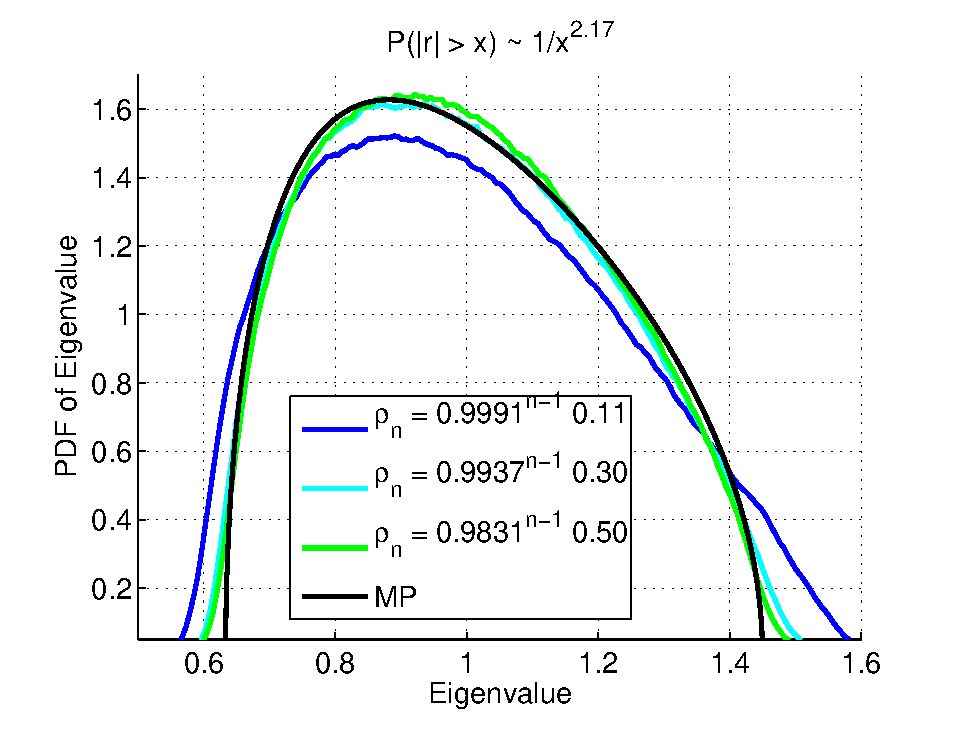
\includegraphics[scale=0.30]{../pics/garch_correlation_eigenvalue_dist_alpha2-17.eps}
    \label{fig:garch2-17_ev_1}
  }
  \subfigure[Tail Exponent 4.00]{
    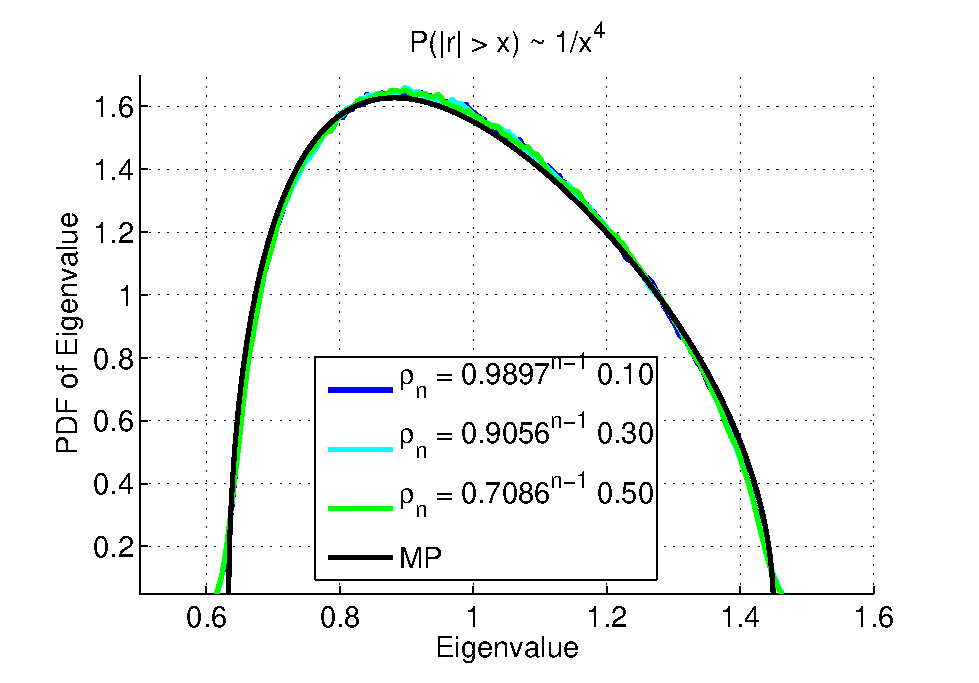
\includegraphics[scale=0.325]{../pics/garch4-00_ev_1.eps}
    \label{fig:garch4-00_ev_1}
  }
  \caption{\small \it Distribution of GARCH correlation matrices'
    eigenvalues. The returns are normalized by sample standard
    deviation and 1/T.}
  \label{fig:garch_ev}
\end{figure}

\begin{figure}[htb!]
  \centering
  \subfigure[PDF]{
    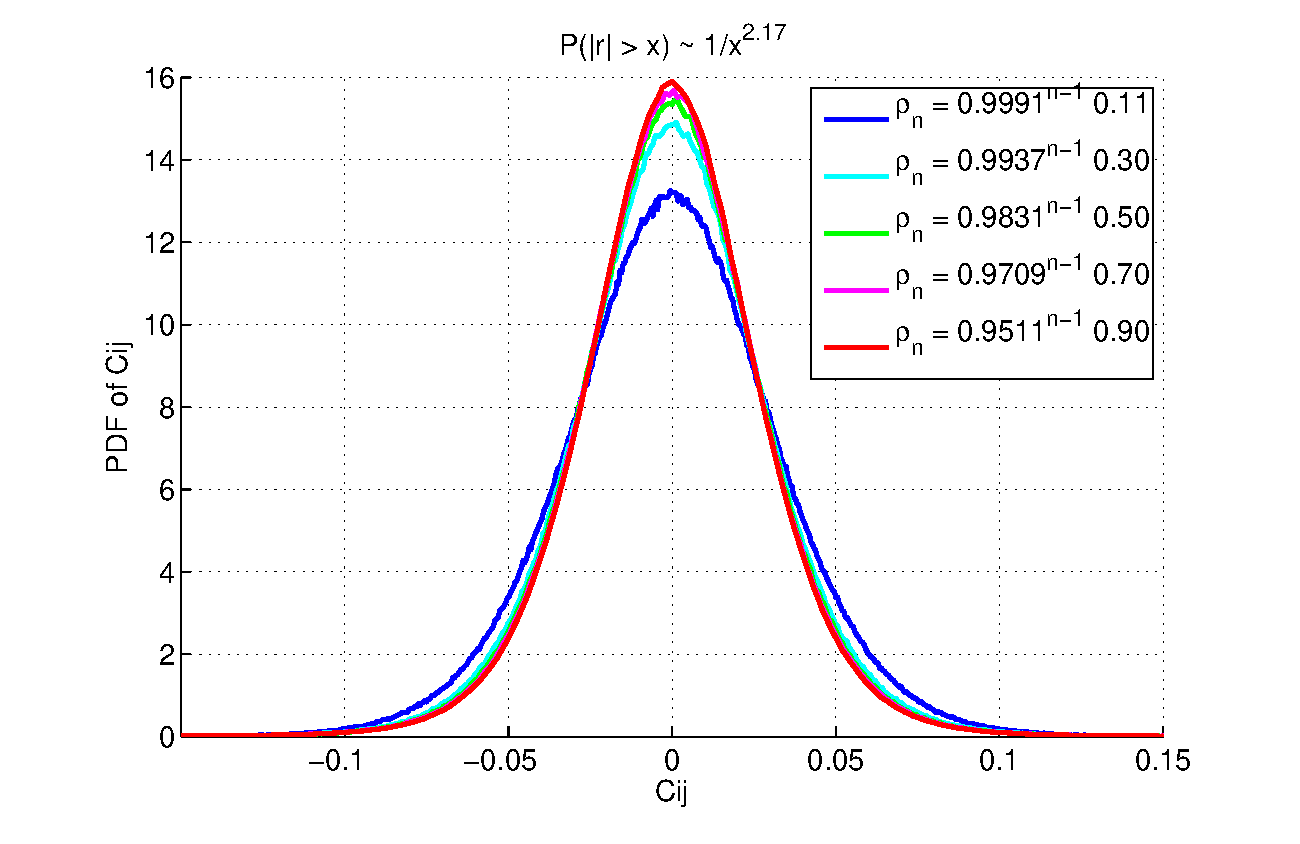
\includegraphics[scale=0.27]{../pics/garch2-17_Cij_1.eps}
    \label{fig:garch2-17_Cij_1}
  }
  \subfigure[$P(C_{ij} > x)$ on log-log scale]{
    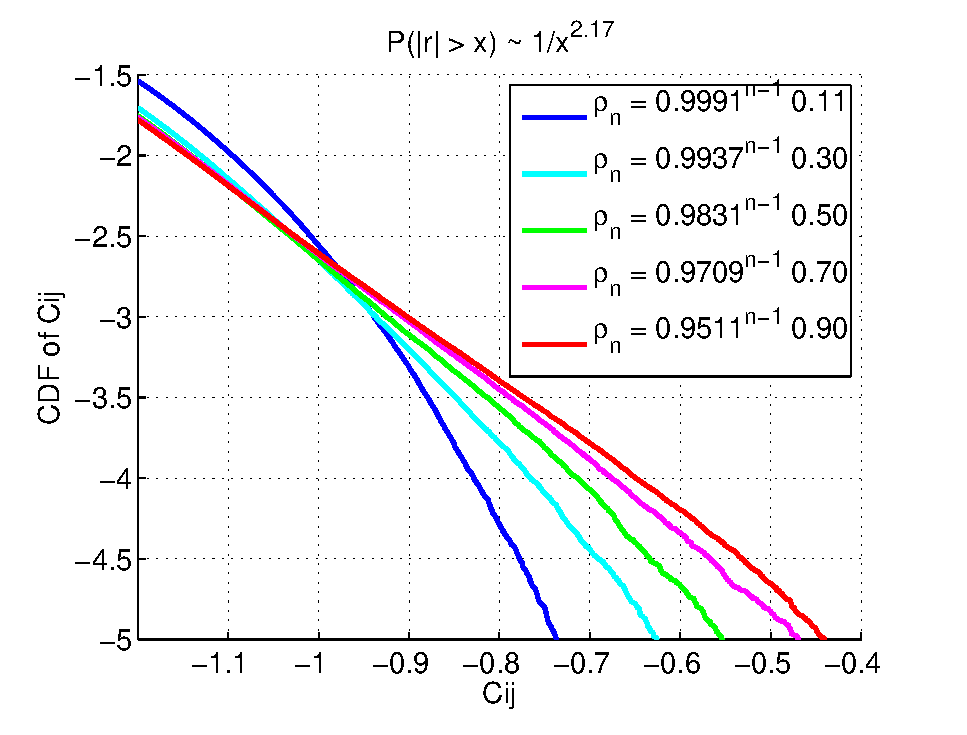
\includegraphics[scale=0.31]{../pics/garch2-17_Cij_2.eps}
    \label{fig:garch2-17_Cij_2}
  }
  \caption{\small \it Distribution of GARCH correlation matrices'
    non-diagonal elements. The returns are normalized by sample
    standard deviation and 1/T. The tail exponent is 2.17.}
  \label{fig:garch_Cij_sample}
\end{figure}

\begin{figure}[htb!]
  \centering
  \subfigure[PDF]{
    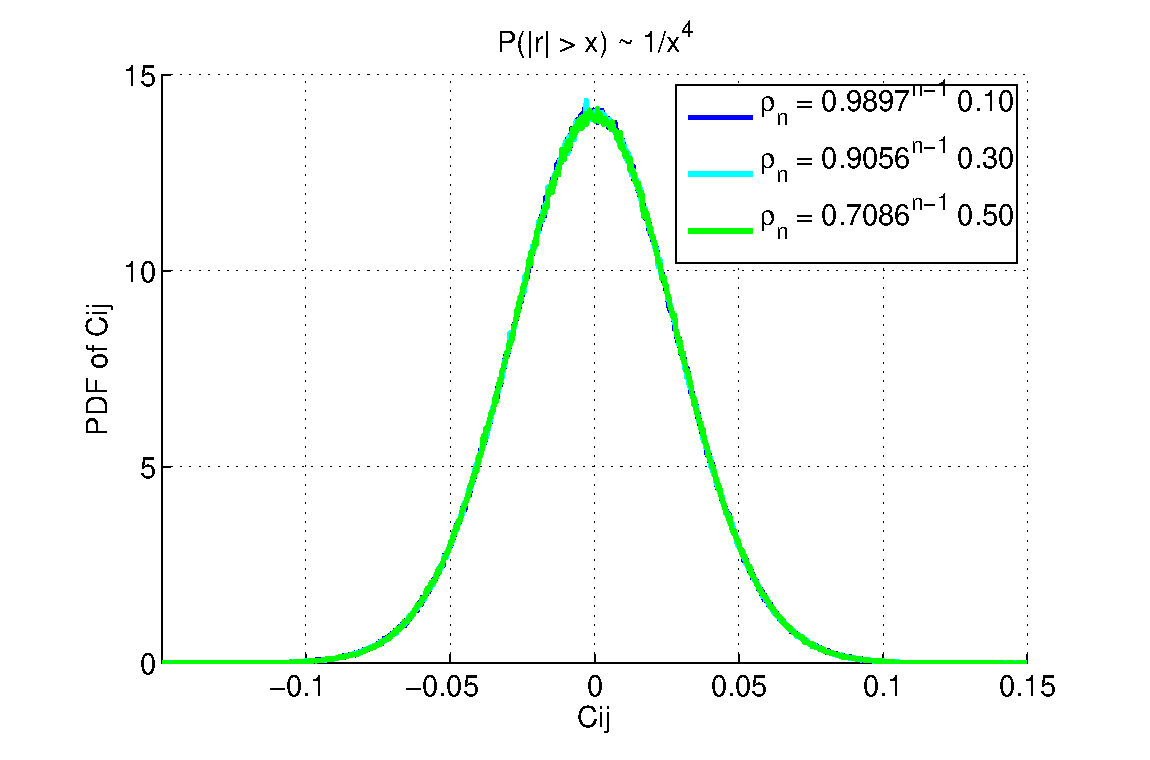
\includegraphics[scale=0.28]{../pics/garch4-00_Cij_1.eps}
    \label{fig:garch4-00_Cij_1}
  }
  \subfigure[$P(C_{ij} > x)$ on log-log scale]{
    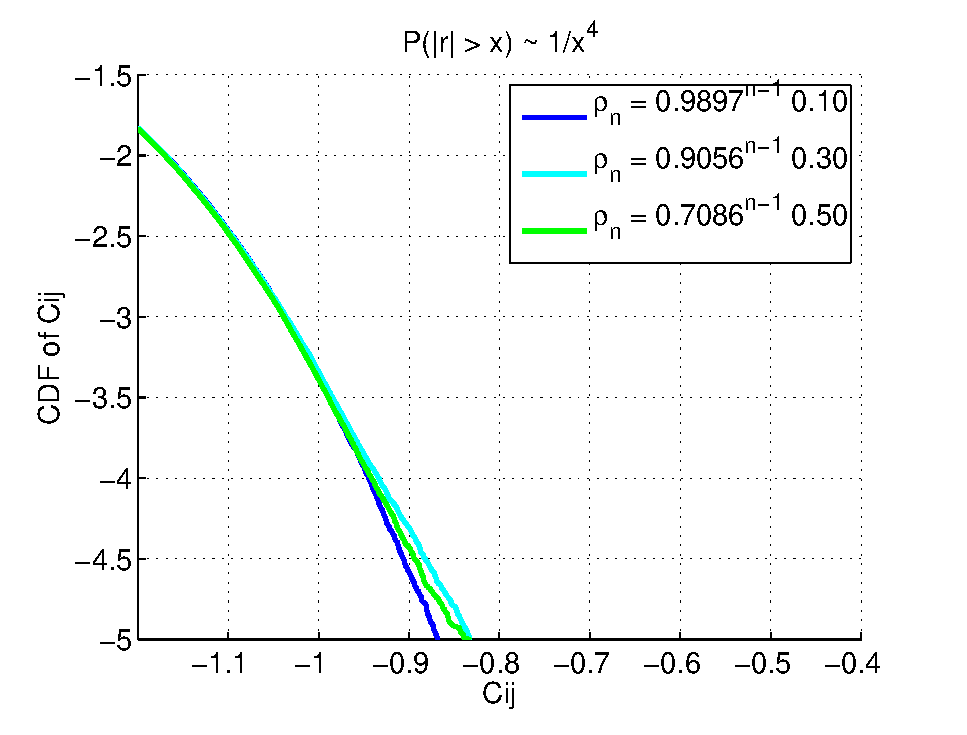
\includegraphics[scale=0.29]{../pics/garch4-00_Cij_2.eps}
    \label{fig:garch4-00_Cij_2}
  }
  \caption{\small \it Distribution of GARCH correlation matrices'
    non-diagonal elements. The returns are normalized by sample
    standard deviation and 1/T. The tail exponent is 4.00.}
  \label{fig:garch_Cij_4.00}
\end{figure}

\begin{figure}[htb!]
  \centering
  \subfigure[PDF]{
    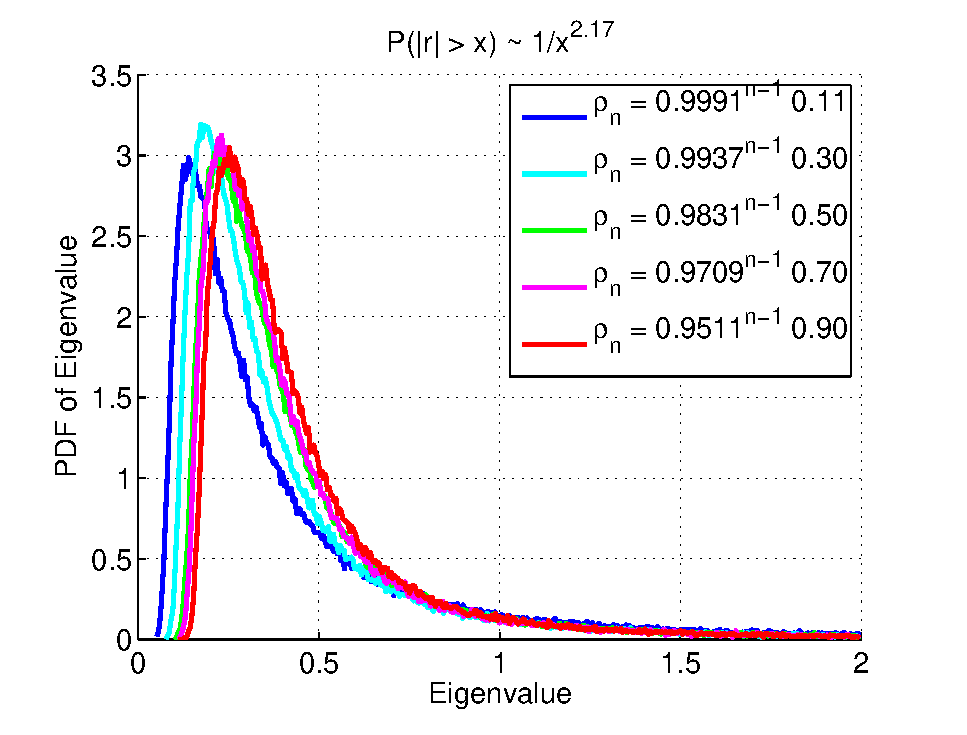
\includegraphics[scale=0.36]{../pics/garch2-17_ev_theo_1.eps}
    \label{fig:garch2-17_ev_theo_1}
  }
  \subfigure[$P(\lambda > x)$ on log-log scale]{
    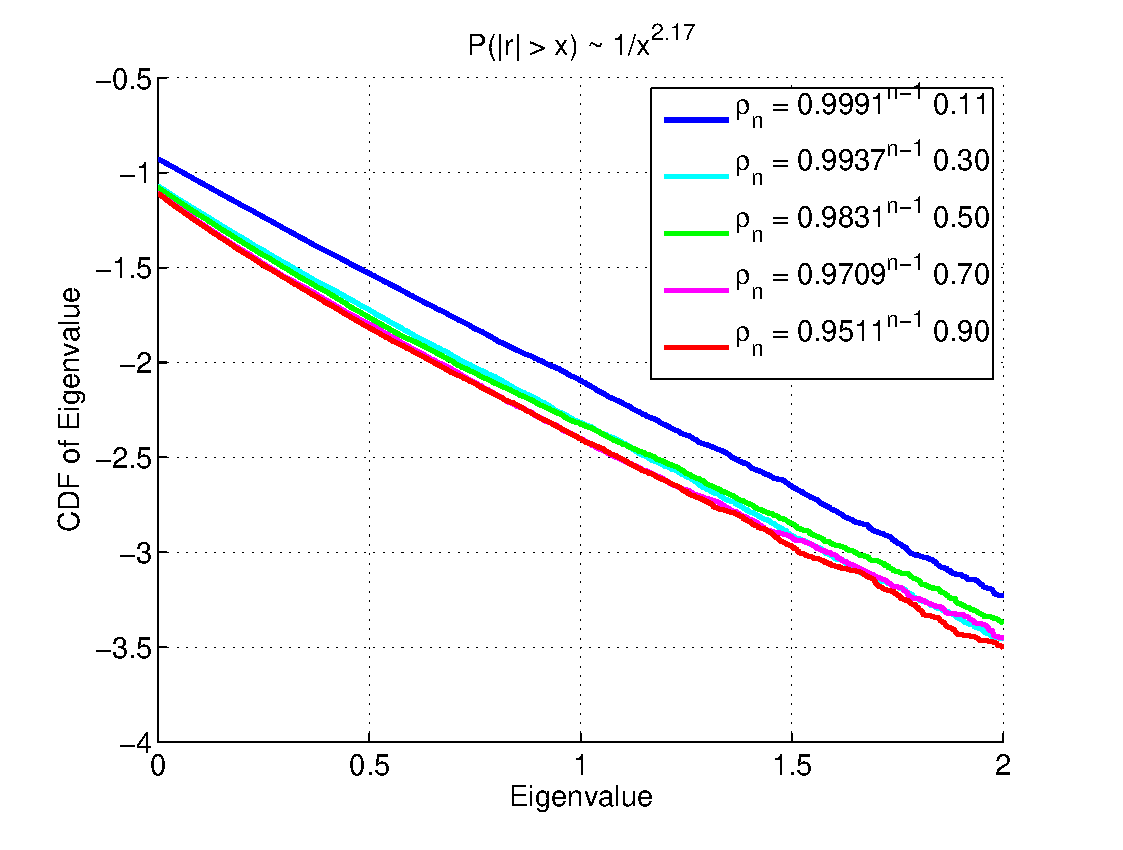
\includegraphics[scale=0.30]{../pics/garch2-17_ev_theo_2.eps}
    \label{fig:garch2-17_ev_theo_2}
  }
  \caption{\small \it Distribution of GARCH correlation matrices'
    eigenvalues. The returns are normalized by theoretical standard
    deviation and 1/T.}
  \label{fig:garch_ev_theo}
\end{figure}

\begin{figure}[htb!]
  \centering
  \subfigure[PDF]{
    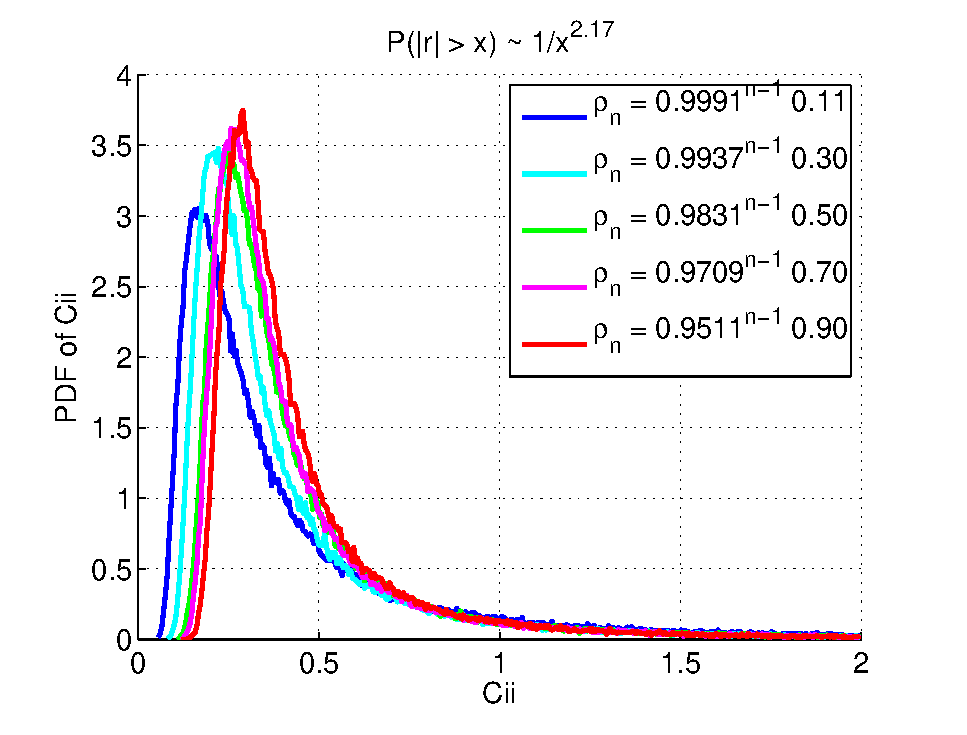
\includegraphics[scale=0.36]{../pics/garch2-17_Cii_theo_1.eps}
    \label{fig:garch2-17_Cii_theo_1}
  }
  \subfigure[$P(C_{ii} > x)$ on log-log scale]{
    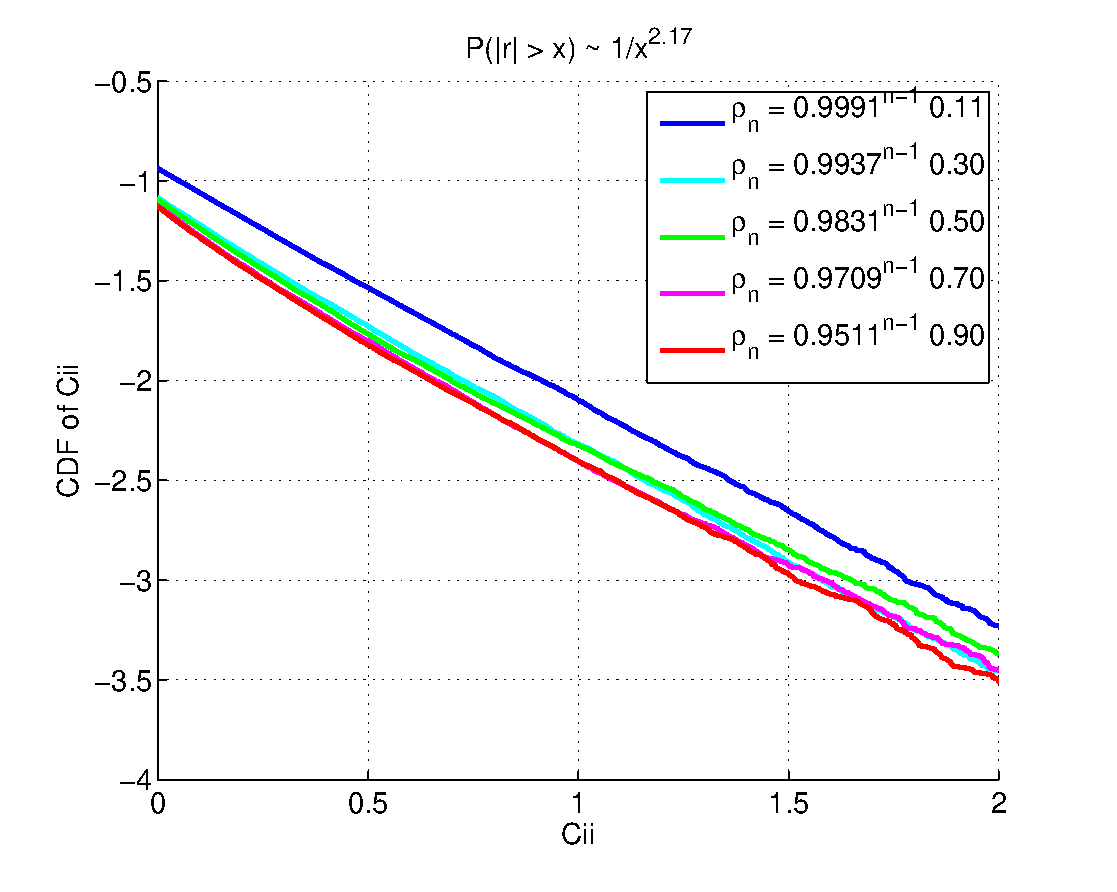
\includegraphics[scale=0.30]{../pics/garch2-17_Cii_theo_2.eps}
    \label{fig:garch2-17_Cii_theo_2}
  }
  \caption{\small \it Distribution of GARCH correlation matrices'
    diagonal elements. The returns are normalized by theoretical standard
    deviation and 1/T.}
  \label{fig:garch_Cii_theo}
\end{figure}

\begin{figure}[htb!]
  \centering
  \subfigure[PDF]{
    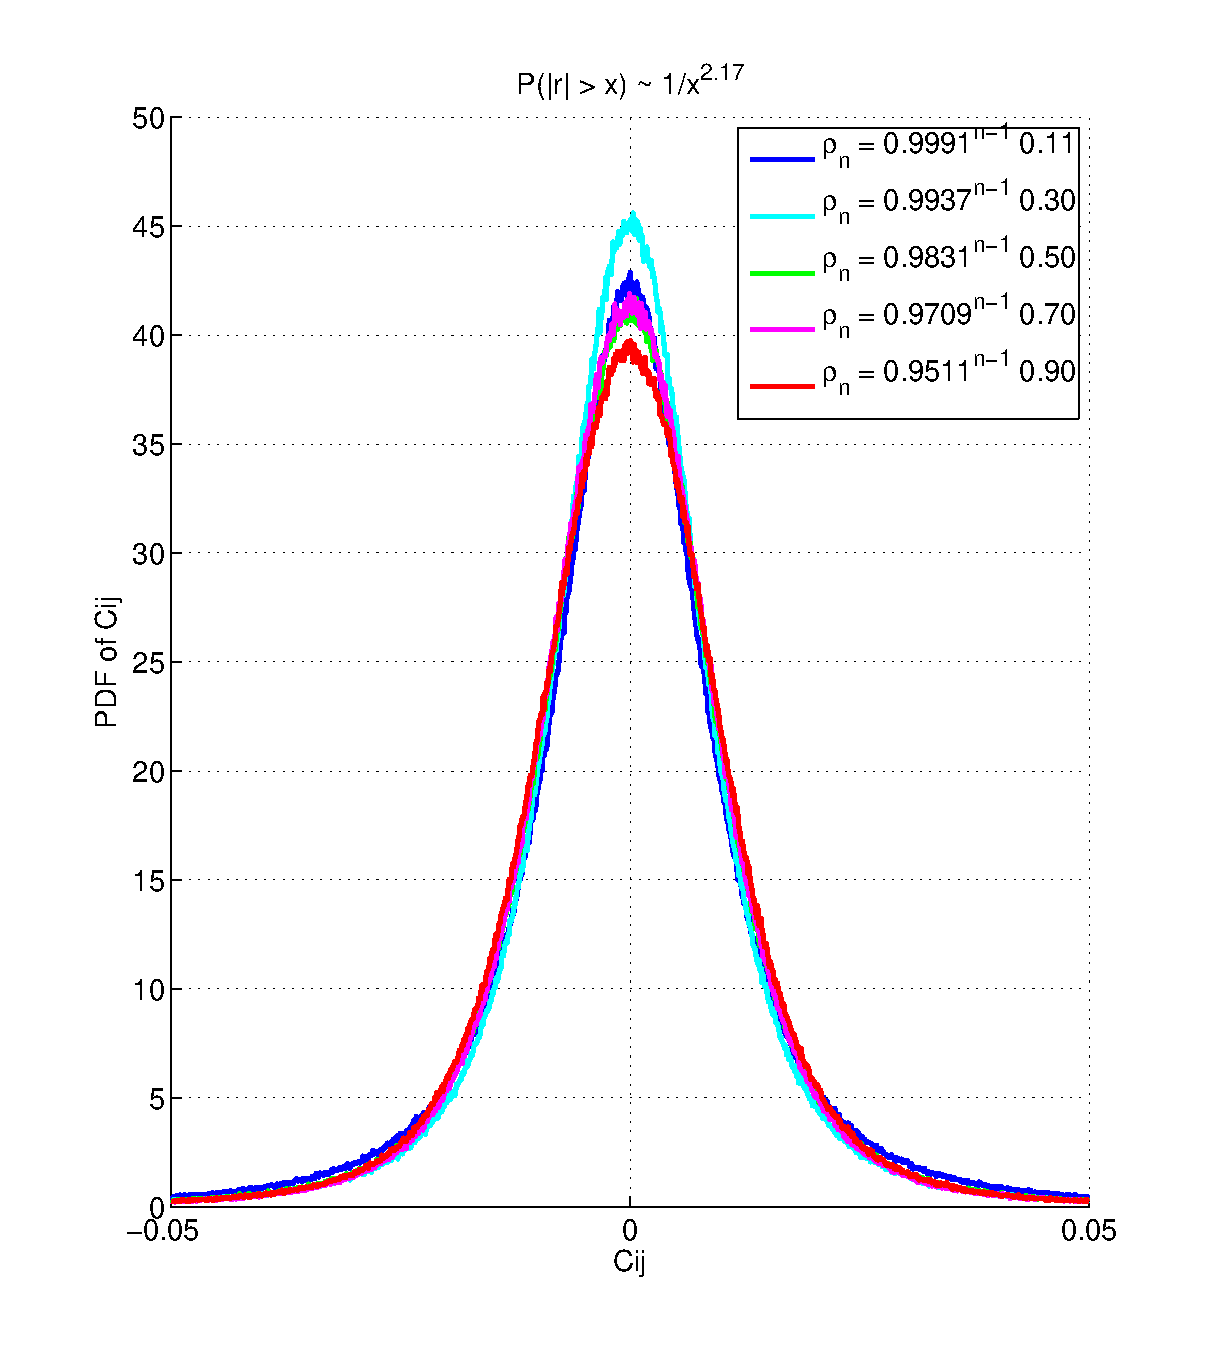
\includegraphics[scale=0.20]{../pics/garch2-17_Cij_3.eps}
    \label{fig:garch2-17_Cij_3}
  }
  \subfigure[$P(C_{ij} > x)$ on log-log scale]{
    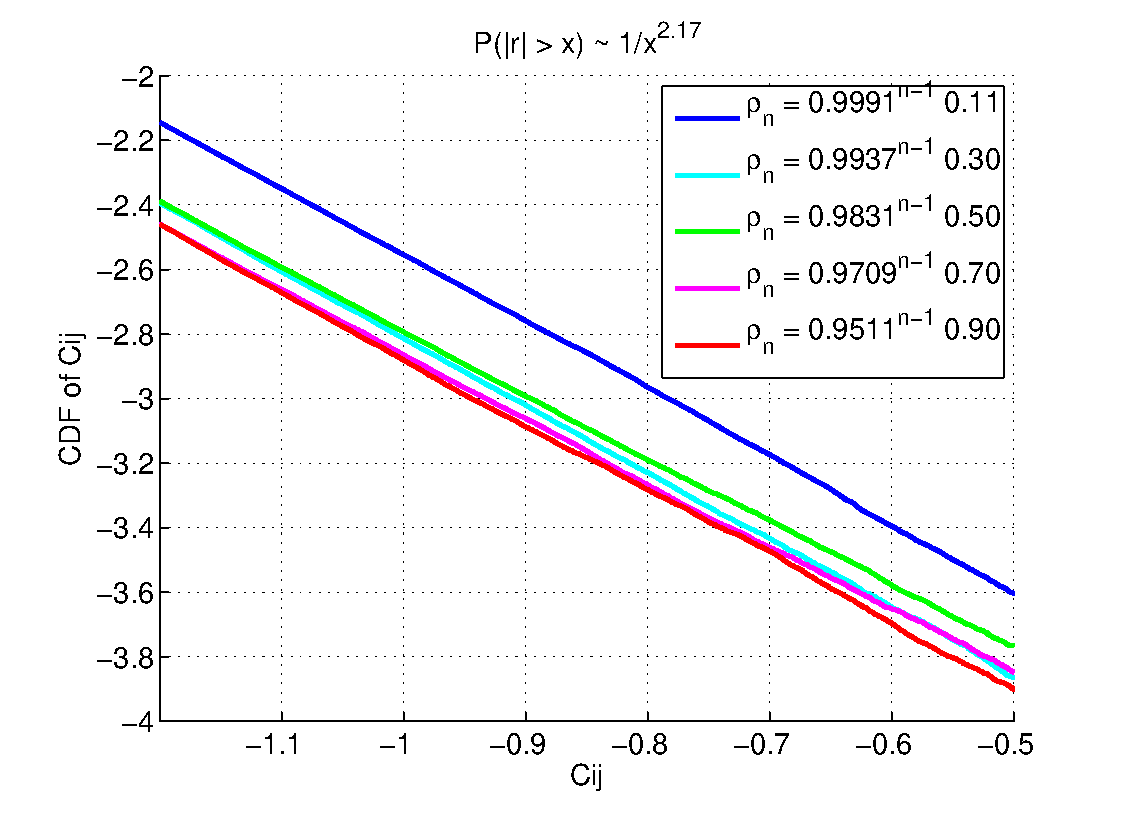
\includegraphics[scale=0.33]{../pics/garch2-17_Cij_4.eps}
    \label{fig:garch2-17_Cij_4}
  }
  \caption{\small \it Distribution of GARCH correlation matrices'
    non-diagonal elements. The returns are normalized by theoretical standard
    deviation and 1/T.}
  \label{fig:garch_Cij_theo}
\end{figure}

\begin{figure}[htb!]
  \centering
  \subfigure[PDF]{
    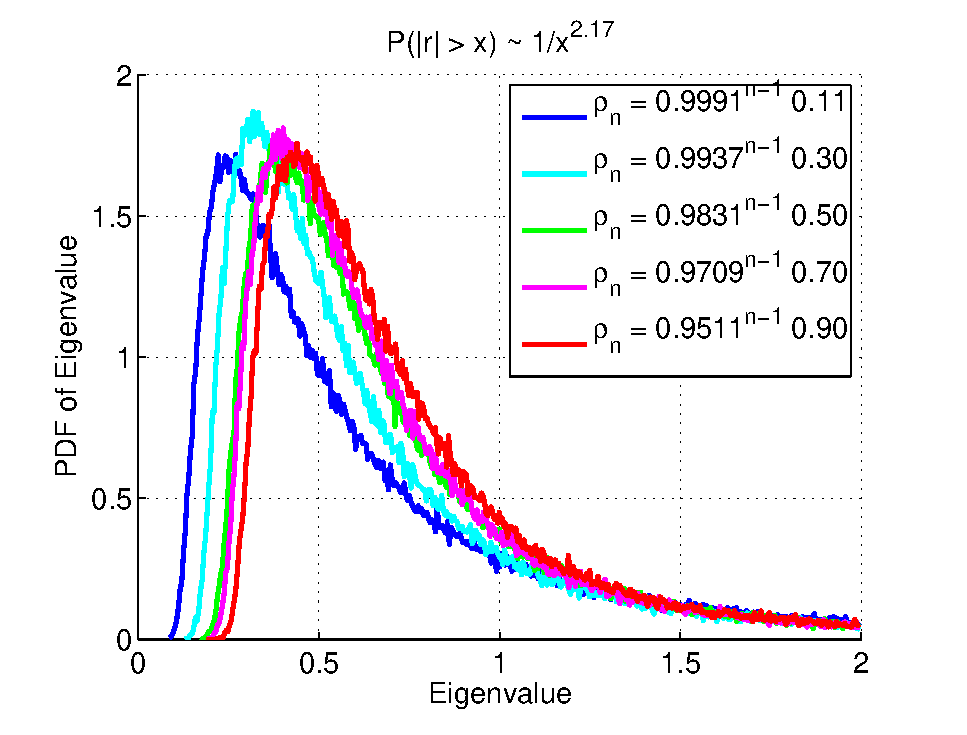
\includegraphics[scale=0.36]{../pics/garch2-17_ev_levy_1.eps}
    \label{fig:garch2-17_ev_levy_1}
  }
  \subfigure[$P(\lambda > x)$ on log-log scale]{
    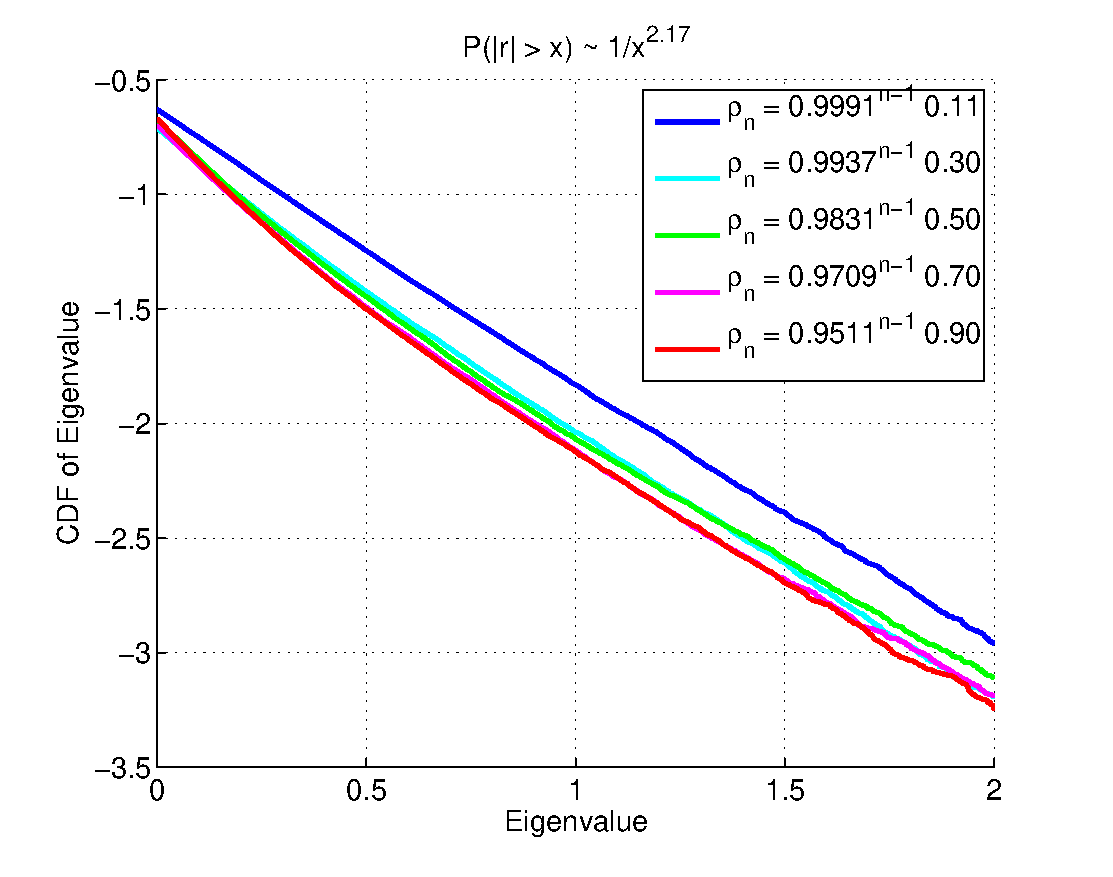
\includegraphics[scale=0.30]{../pics/garch2-17_ev_levy_2.eps}
    \label{fig:garch2-17_ev_levy_2}
  }
  \caption{\small \it Distribution of GARCH correlation matrices'
    Eigenvalues. The returns are normalized by $1/T^{2/\alpha}$.}
  \label{fig:garch_ev_levy}
\end{figure}

\begin{figure}[htb!]
  \centering
  \subfigure[PDF]{
    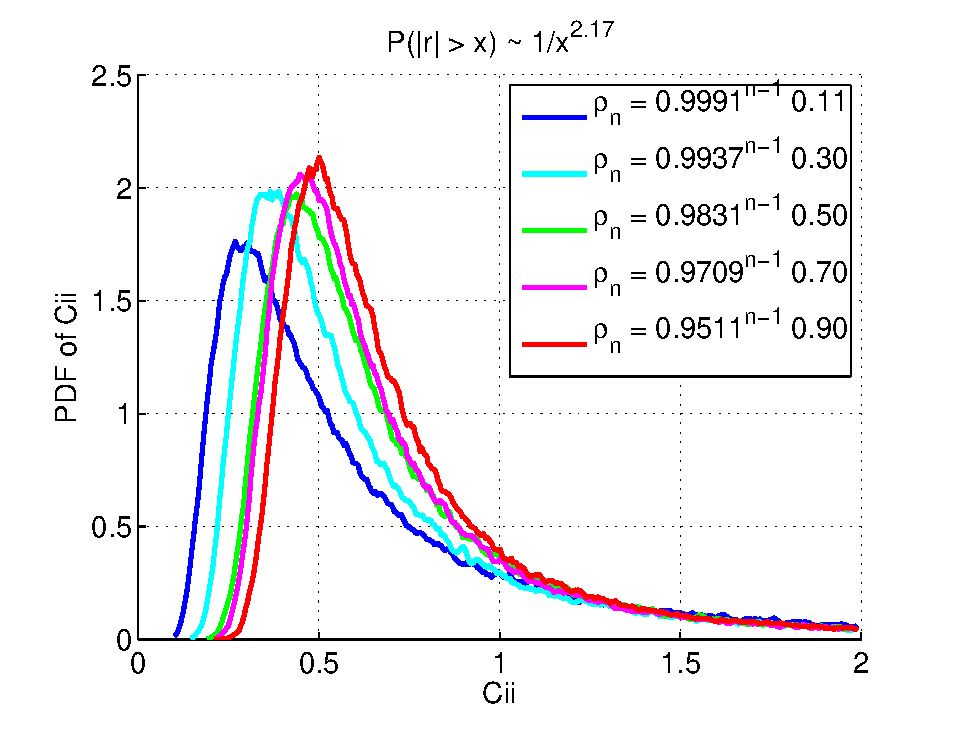
\includegraphics[scale=0.36]{../pics/garch2-17_Cii_levy_1.eps}
    \label{fig:garch2-17_Cii_levy_1}
  }
  \subfigure[$P(C_{ii} > x)$ on log-log scale]{
    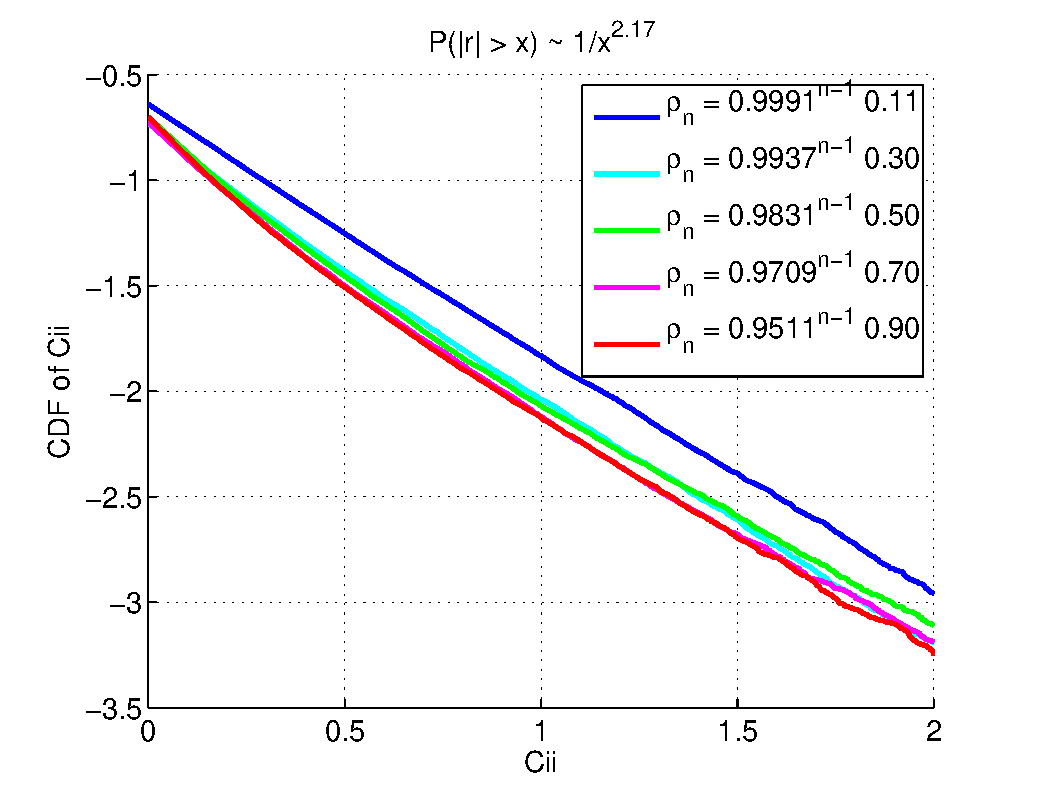
\includegraphics[scale=0.30]{../pics/garch2-17_Cii_levy_2.eps}
    \label{fig:garch2-17_Cii_levy_2}
  }
  \caption{\small \it Distribution of GARCH correlation matrices'
    diagonal elements. The returns are normalized by
    $1/T^{2/\alpha}$.}
  \label{fig:garch_Cii_levy}
\end{figure}

\begin{figure}[htb!]
  \centering
  \subfigure[PDF]{
    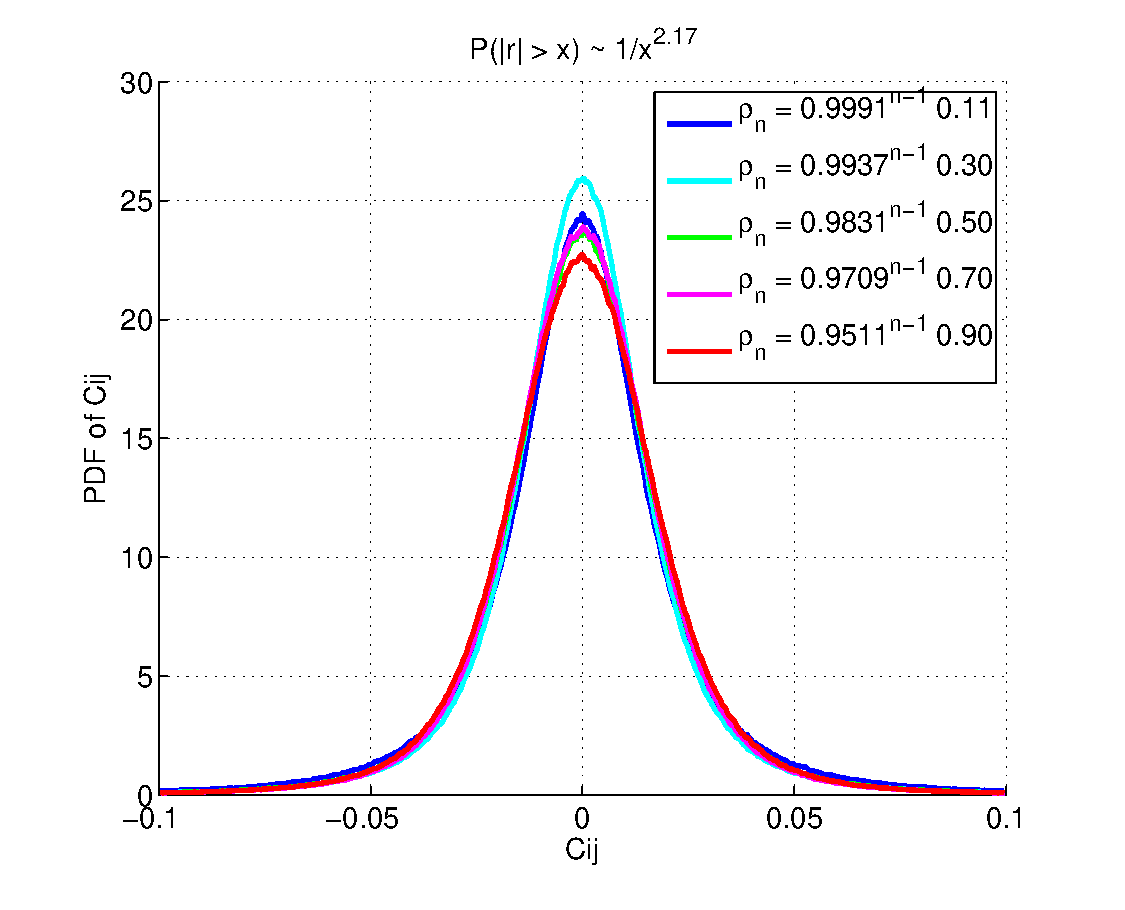
\includegraphics[scale=0.26]{../pics/garch2-17_Cij_levy_1.eps}
    \label{fig:garch2-17_Cij_levy_1}
  }
  \subfigure[$P(C_{ij} > x)$ on log-log scale]{
    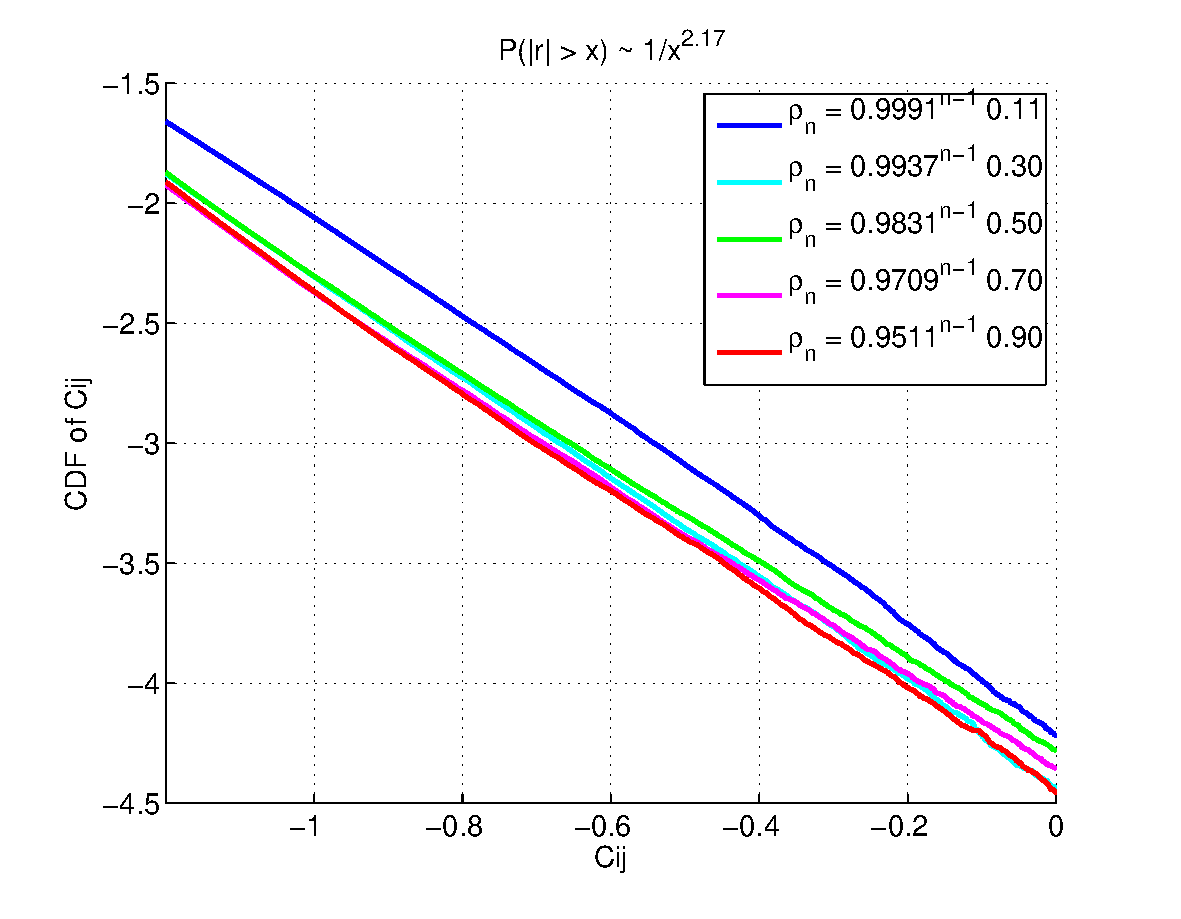
\includegraphics[scale=0.25]{../pics/garch2-17_Cij_levy_2.eps}
    \label{fig:garch2-17_Cij_levy_2}
  }
  \caption{\small \it Distribution of GARCH correlation matrices'
    non-diagonal elements. The returns are normalized by
    $1/T^{2/\alpha}$.}
  \label{fig:garch_Cij_levy}
\end{figure}



\end{document}
